\documentclass{article}

\usepackage{comment}
\usepackage{amsmath}
\usepackage{natbib}
\usepackage{listings}
\usepackage{subfig}
\usepackage{color}
\usepackage{etoolbox}
\usepackage{tikz}
\usepackage{boxedminipage}
\usetikzlibrary{decorations.pathreplacing,calc}
\usetikzlibrary{positioning,shadows,arrows}

\newcommand{\pdfauthors}{Chris Fournier}
\newcommand{\pdftitle}{Segmentation Representation Specification}
\newcommand{\pdfversion}{Version 1.0.2}

% Set up hyperlinks
\usepackage[pdfauthor={\pdfauthors},%
pdftitle={\pdftitle},%
pdfborder=0 0 0,
pdftex]{hyperref}

\hypersetup{ 
colorlinks,% 
citecolor=black,% 
filecolor=black,% 
linkcolor=black,% 
urlcolor=black 
}

\colorlet{block_norm}{gray!15}
% TikZ styles
\tikzstyle{header}=[draw, rectangle, minimum width=1.25em, minimum height=1.25em, anchor=south west]
\tikzstyle{block}=[draw, rectangle, minimum width=1.25em, minimum height=1.25em, fill=block_norm, anchor=south west]
\tikzstyle{header_bound}=[draw=none, minimum width=1.25em, minimum height=1.25em, anchor=south west, xshift=-0.4em, yshift=1em]
\tikzstyle{bound}=[draw=none, minimum width=1.25em, minimum height=1.25em, anchor=south west]
\tikzstyle{leveltag}=[rectangle, draw=none, rounded corners=1mm, fill=gray, text centered, anchor=north, text=white]

% TiKZ commands
\newcommand{\segmentationA}[2]{
\node[header] (a0) at (0,0) {#1};
  \xdef\lasti{0}
  \foreach [count=\i, remember=\i as \lasti] \x in {#2} {
    \node[block, minimum width=\x * 1.25 em] (a\i) [right=of a\lasti] {$\x$};
  }
}
\newcommand{\segmentationB}[1]{
\node[header] (b0) [below=of a0] {$s_2$};
  \xdef\lasti{0}
  \foreach [count=\i, remember=\i as \lasti] \x in {#1} {
    \node[block, minimum width=\x * 1.25 em] (b\i) [right=of b\lasti] {$\x$};
  }
}
\newcommand{\segmentationLabels}[1]{
\node[header_bound] (c0) [above=of a0] {};
  \xdef\lasti{0} %
  \foreach \xa/\xb/\xc/\xd/\xe [count=\i, remember=\i as \lasti] in {#1} {
    \node[bound] (c\i) [right=of c\lasti] {
    \begin{minipage}[b][3em]{0.5em}
    \centering
      \ifdefempty{\xe}{}{\xe \\}
      \ifdefempty{\xd}{}{\xd \\}
      \ifdefempty{\xc}{}{\xc \\}
      \ifdefempty{\xb}{}{\xb \\}
      \ifdefempty{\xa}{}{\xa}
    \end{minipage}
    };
  }
}
\newcommand{\segmentationLowerLabels}[1]{
\node[header_bound, yshift=-2em] (c0) [below=of a0] {};
  \xdef\lasti{0} %
  \foreach \xa/\xb/\xc/\xd/\xe [count=\i, remember=\i as \lasti] in {#1} {
    \node[bound] (c\i) [right=of c\lasti] {
    \begin{minipage}[t][3em]{0.5em}
    \centering
      \ifdefempty{\xe}{}{\xe \\}
      \ifdefempty{\xd}{}{\xd \\}
      \ifdefempty{\xc}{}{\xc \\}
      \ifdefempty{\xb}{}{\xb \\}
      \ifdefempty{\xa}{}{\xa}
    \end{minipage}
    };
  }
}
\newcommand{\boundariesOne}[1]{
  $
  \foreach \xa/\xb/\xc/\xd/\xe in {#1} {
    \{
      \ifdefempty{\xa}{{\color{white}0}}{\xa}
      \ifdefempty{\xb}{}{,\xb}
      \ifdefempty{\xc}{}{,\xc}
      \ifdefempty{\xd}{}{,\xd}
      \ifdefempty{\xe}{}{,\xe}
    \}
  }
  $
}

% listings settings
\lstset{ %
  language=,                % the language of the code
  basicstyle=\footnotesize,           % the size of the fonts that are used for the code
  numbers=left,                   % where to put the line-numbers
  numberstyle=\tiny\color{gray},  % the style that is used for the line-numbers
  stepnumber=1,                   % the step between two line-numbers. If it's 1, each line 
                                  % will be numbered
  numbersep=5pt,                  % how far the line-numbers are from the code
  backgroundcolor=\color{white},      % choose the background color. You must add \usepackage{color}
  showspaces=false,               % show spaces adding particular underscores
  showstringspaces=false,         % underline spaces within strings
  showtabs=false,                 % show tabs within strings adding particular underscores
  frame=single,                   % adds a frame around the code
  rulecolor=\color{black},        % if not set, the frame-color may be changed on line-breaks within not-black text (e.g. commens (green here))
  tabsize=2,                      % sets default tabsize to 2 spaces
  captionpos=b,                   % sets the caption-position to bottom
  breaklines=true,                % sets automatic line breaking
  breakatwhitespace=false,        % sets if automatic breaks should only happen at whitespace
  title=\lstname,                   % show the filename of files included with \lstinputlisting;
                                  % also try caption instead of title
  keywordstyle=\color{blue},          % keyword style
  commentstyle=\color{dkgreen},       % comment style
  stringstyle=\color{mauve},         % string literal style
  escapeinside={\%*}{*)},            % if you want to add a comment within your code
  morekeywords={*,...}               % if you want to add more keywords to the set
}

% Custom commands
\def\citeapos#1{\citeauthor{#1}'s (\citeyear{#1})}

\begin{document}



\title{\pdftitle
\\
{\large \pdfversion}}
\author{\pdfauthors}
\date{\today}
\maketitle



\section{Introduction}
``Segmentation is the task of splitting up an item, such as a document,
into a sequence of segments by placing boundaries within. The purpose of
segmenting can vary greatly, but one common objective is to denote shifts in the
topic of a text...''~\citep{FournierInkpen2012}.  In this document, the process
and file format for storing segmentations of varying types is detailed.



\section{Representations}
In addition to the conceptualizations presented, each segmentation
representation is to be stored  as UTF-8 encoded text files in either the TSV
(tab separated values) format, or in the JSON (JavaScript Object Notation)
format.  

JSON is an ideal file format because it allow for the encoding of key/value
pairs and lists.  Sequences of internal segments, or boundaries, are easily
stored as lists, and metadata about the type of segmentation performed can be
stored in key/value pairs, and nested key/value pairs can be used to store
multiple segmentations (produced under the same conditions) by coders in the
same file.  JSON metadata common to all representations is shown in
Figure~\ref{fig:json} with ``\verb+|+'' characters representing the available
options for a field, and ``\verb+*+'' representing an optional field whose
first options is assumed to be the default.

\begin{figure}[h]
\begin{lstlisting}[language=]
{
	"segmentation_type" : "linear"|"multiple"|"hierarchical",
	"items" : {...},
	"*has_reference_coder": "false"|"true"
}
\end{lstlisting}
\vspace{-3em}
\caption{Common JSON segmentation structure}
\label{fig:json}
\end{figure}

The \verb+has_reference_coder+ property indicates that the file contains a coder
named \verb+reference+ who represents a single, authoritative, reference coder,
to which all other coders can be compared against to compute S-based precision,
recall, and $\text{F}_{\beta}\text{-measure}$.  If more than one reference 
coding is possible for a single item, it can be denoted as coder
\verb+reference+, \verb+reference2+, \verb+reference3+, etc.


\subsection{Linear Segmentation}
The simplest case of linear segmentation is the segmentation of text by placing
only one type boundary inside a text to split it into a number of internal
segments whose whole is called a \emph{segmentation}.

To illustrate this, let's go through a contrived example to produce a
line-level\footnote{This is a segmentation's \emph{granularity}; common choices
are sentence or paragraph levels.} segmentation of an excerpt of
\citeapos{Coleridge1816} poem titled Kubla Khan \citep[pp.
55--58]{Coleridge1816}, shown below in Figure~\ref{fig:linear:text:kublakhan}.

\begin{figure}[h]
\begin{lstlisting}[language=]
In Xanadu did Kubla Khan
A stately pleasure-dome decree:
Where Alph, the sacred river, ran
Through caverns measureless to man
Down to a sunless sea.
So twice five miles of fertile ground
With walls and towers were girdled round:
And here were gardens bright with sinuous rills,
Where blossomed many an incense-bearing tree;
And here were forests ancient as the hills,
Enfolding sunny spots of greenery.
\end{lstlisting}
\vspace{-3em}
\caption{Excerpt from Kubla Khan \citep[pp. 55--58]{Coleridge1816}}
\label{fig:linear:text:kublakhan}
\end{figure}

If a person was to topically segment the previous excerpt, they may choose
to group the lines together (with a short description of the internal segment)
as shown in Figure~\ref{fig:linear:segmentation:kublakhan}.

\begin{figure}[h]
\centering
\begin{tabular}{ r l }
\textbf{Lines}  & \textbf{Description} \\ \hline \hline
1--2  & Kubla Khan and his decree \\
3--5  & Waterways \\
6--11 & Fertile ground and greenery \\
\end{tabular}
\caption{Hypothetical line-level segmentation of the excerpt in Figure~\ref{fig:linear:text:kublakhan}}
\label{fig:linear:segmentation:kublakhan}
\end{figure}

The previous hypothetical segmentation is essentially a sequence of internal
segments, each with a size (i.e., \emph{mass}) defined as:

\begin{equation}\label{eqn:linear:pos}
\text{mass}(segment) = \text{position}(segment_{end}) - \text{position}(segment_{start}) + 1
\end{equation}
\vspace{0.00em}

If we apply this function to the positions of each internal segment, we can
represent the segmentation as a sequence of masses:

\begin{equation}\label{eqn:linear:seq}
2,3,6
\end{equation}
\vspace{0.00em}

We can represent this sequence of internal segment masses graphically as shown
in Figure~\ref{fig:linear:segmentation:graphic:kublakhan}.

\begin{figure}[h]
\centering
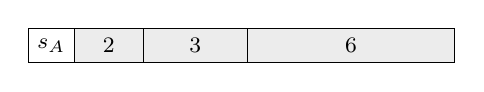
\begin{tikzpicture}[node distance=0cm, outer sep=0pt, font=\footnotesize]
  \segmentationA{$s_A$}{2,3,6}
\end{tikzpicture}
\caption{Hypothetical line-level segmentation of the excerpt in Figure~\ref{fig:linear:text:kublakhan}}
\label{fig:linear:segmentation:graphic:kublakhan}
\end{figure}

To store this sequence of internal segment masses, we can simply store the
sequence shown in Equation~\ref{eqn:linear:seq} inside a file.  We will often
have multiple segmentation of the same text (e.g.,
Table~\ref{table:linear:multiple_segmentations:kublakhan}), however, so it would
be useful to store all segmentations of the same text inside the same file, with
the name of the \emph{coder} (i.e., person who created the segmentation) to be
able to cross-reference this person's segmentations across multiple files.

\begin{table}[h]
\centering
\begin{tabular}{ r l }
\textbf{Coder}  & \textbf{Segmentation} \\ \hline \hline
A & $2,3,6$ \\
B & $1,1,3,6$ \\
C & $2,3,2,4$ \\
\end{tabular}
\caption{Hypothetical line-level segmentations of the excerpt in Figure~\ref{fig:linear:text:kublakhan}}
\label{table:linear:multiple_segmentations:kublakhan}
\end{table}

To store the segmentations shown in
Table~\ref{table:linear:multiple_segmentations:kublakhan}, we can store the
sequences of internal segment masses per coder, as shown in
Figure~\ref{fig:linear:segmentation:files}.

\newsavebox{\lineartsv}
\begin{lrbox}{\lineartsv}
\begin{minipage}[b]{0.5\textwidth}
\begin{lstlisting}[language=,linewidth=0.9\textwidth]
Coder	Masses
A	2	3	6
B	1	1	3	6
C	2	3	2	4

\end{lstlisting}
\vspace{-2em}
\end{minipage}
\end{lrbox}

\newsavebox{\linearjson}
\begin{lrbox}{\linearjson}
\begin{minipage}[b]{0.5\textwidth}
\begin{lstlisting}[language=,linewidth=0.9\textwidth]
{
	"segmentation_type" : "linear"
	"items" :
	{
		"Kubla Khan" : {
			"A" : [2,3,6],
			"B" : [1,1,3,6],
			"C" : [2,3,2,4]
		}
	}
}
\end{lstlisting}
\vspace{-2em}
\end{minipage}
\end{lrbox}

\begin{figure}[h]
\hspace{1em}
\subfloat[TSV]{\usebox{\lineartsv}}
\subfloat[JSON]{\usebox{\linearjson}}
\caption{File representations of the hypothetical segmentations in Table~\ref{table:linear:multiple_segmentations:kublakhan}}
\label{fig:linear:segmentation:files}
\end{figure}

In JSON files, multiple items can be added to the same file to represent a
data set.  In this case, all of the coder names across items are assumed to
refer to the same coder, so that overall statistics can be calculated for a
data set.


\section{Future Work}
Future versions of this specification will include additional formats as support
for them are added to the \texttt{\href{http://nlp.chrisfournier.ca/software/}{segeval}}
python package, including:
\begin{enumerate}
  \setlength{\itemsep}{0cm}%
  \setlength{\parskip}{0cm}%
  \item Linear Segmentation with Multiple Boundary Types, with:
  \begin{itemize}
    \item Categorical or ordinal boundaries;
    \item Mutually exclusive or non-exclusive sets of boundary positions;
  \end{itemize}
  \item Hierarchical Segmentation.
\end{enumerate}


\addcontentsline{toc}{chapter}{References}
\bibliographystyle{agsm} % Harvard = agsm
\bibliography{bib/resources}

\end{document}





